\begin{figure}[htbp]
\centering
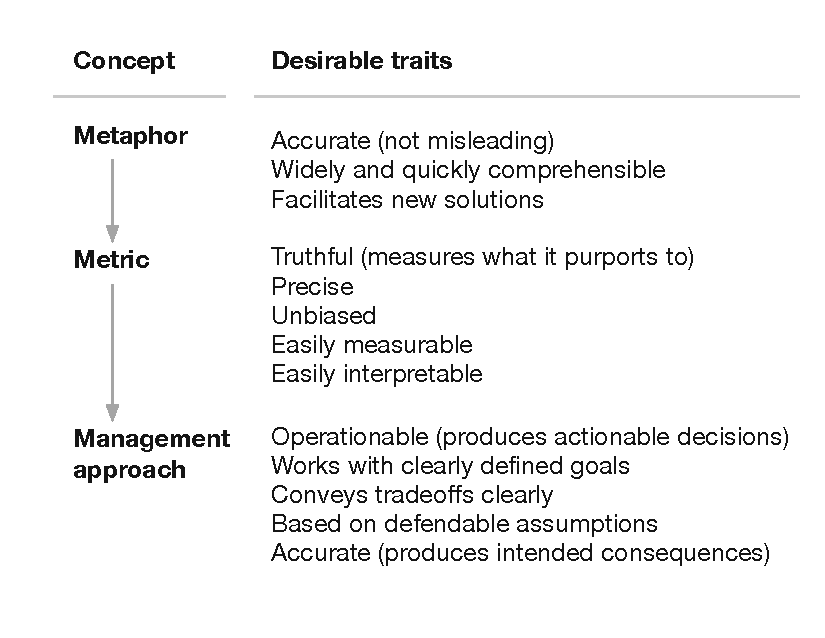
\includegraphics[width=4in]{mmm-traits.pdf}
\caption{
Desirable traits of ecological metaphors, metrics, and management approaches
(decision-making tools).
}
\label{fig:traits}
\end{figure}

\clearpage

\begin{figure}[htbp]
\centering
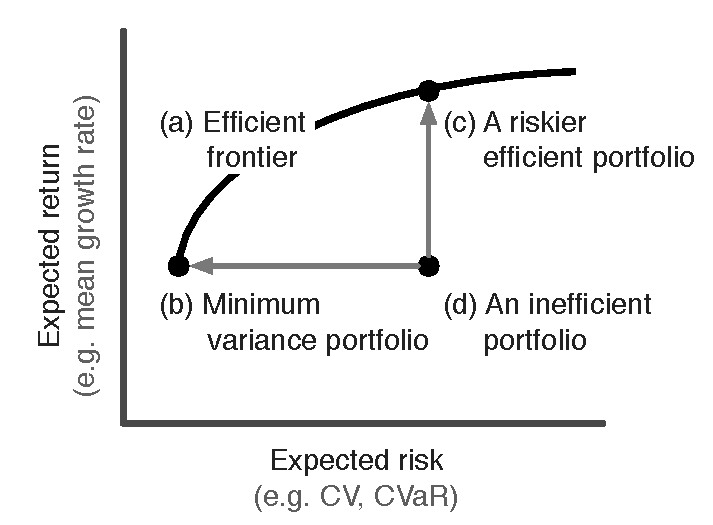
\includegraphics[width=3in]{efficient-frontier-fig.pdf}
\caption{
An introduction to Modern Portfolio Theory mean-variance optimization. In
finance, portfolios are formed by choosing how much to invest in various
assets. Modern Portfolio Theory focuses on identifying the set of portfolios
that optimizes the trade-off between expected return (mean) and expected
variance or risk. (a) This set of portfolios is referred to as the efficient
frontier. (b) The minimum variance portfolio achieves the lowest expected
risk; the remaining risk is said to be undiversifiable. (c) A risker, but
still efficient portfolio. (d) An example inefficient portfolio, which has a
lower expected return than (c) and greater expected risk than (b). Adapted
from \citeauthor{hoekstra2012} (\citeyear{hoekstra2012}).
}
\label{fig:mpt}
\end{figure}

\clearpage

% \begin{figure}[htbp]
% \centering
% 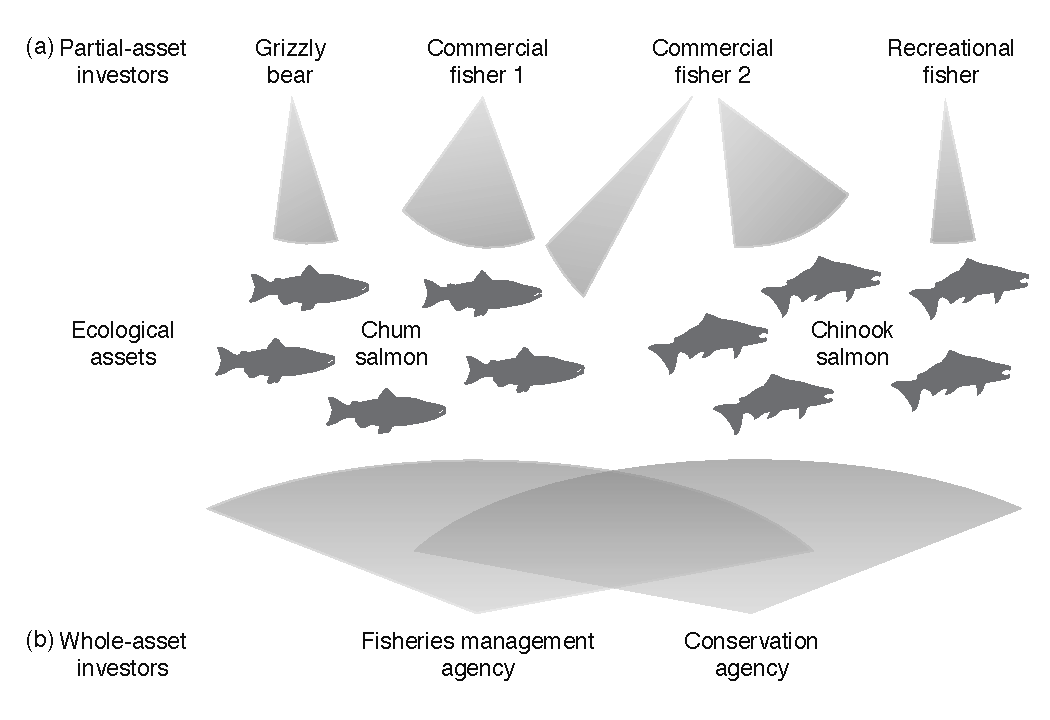
\includegraphics[width=4.2in]{salmon-portfolios-bw.pdf}
% \caption{
% There are multiple ways of investing in ecological portfolios. In this
% example, investors are shown along the top and bottom and ecological assets
% are shown in the middle (populations of chum salmon, \emph{Oncorhynchus keta},
% and Chinook salmon, \emph{Oncorhynchus tshawytscha}). The shaded arcs indicate
% investment. (a) Partial-asset investors invest by removing portions of the
% salmon populations --- the salmon that commercial fisher 1 removes are
% unavailable for the grizzly bear. These investors can often change their
% investment with ease. For example, commercial fisher 2 could decide to fish
% more Chinook and less chum salmon. Most financial portfolio theory is
% developed around this paradigm. (b) Whole-asset investors invest in entire
% populations. These investors can share assets but may have different goals for
% their portfolio. They can adjust their investment by managing properties of
% the population itself. For example, the fisheries management agency could
% reduce fishing of chum salmon to allow the population to grow. The
% conservation agency could fund habitat restoration for Chinook salmon to
% increase carrying capacity and expand their investment.
% }
% \label{fig:salmonport}
% \end{figure}

\begin{figure}[htbp]
\centering
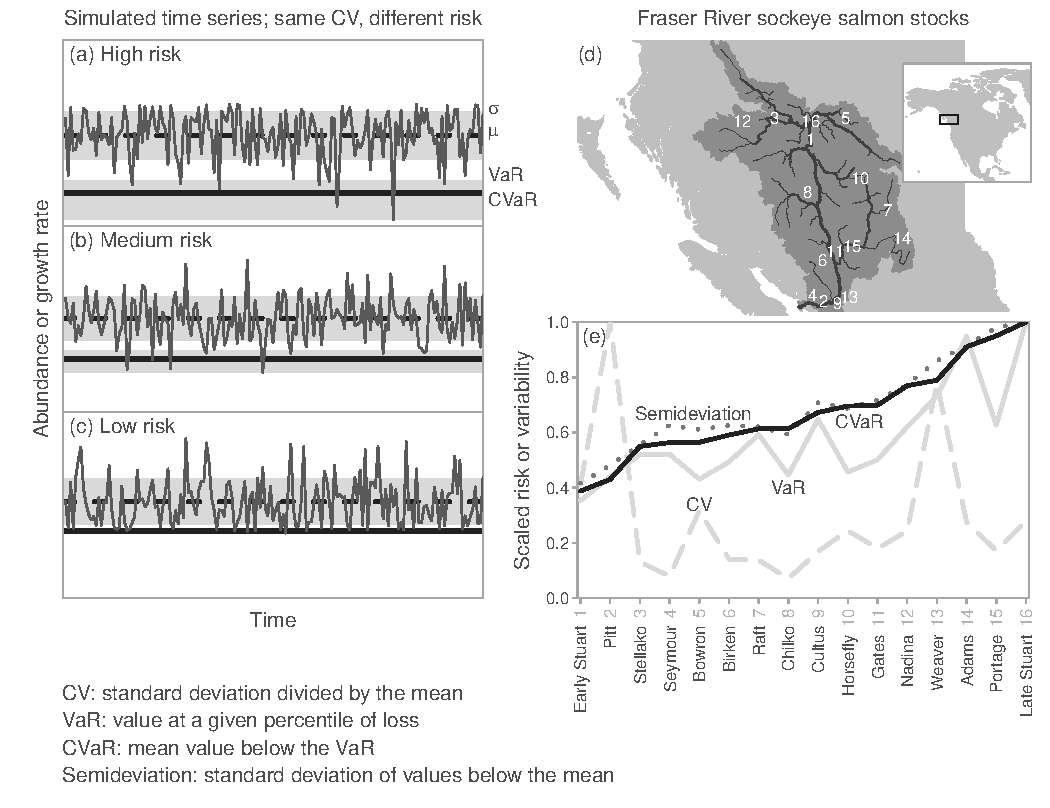
\includegraphics[width=5.5in]{risk-fig/risk-fig-bw.pdf}
\caption{
Symmetric variability vs.~downside risk metrics. (a--c) An illustration of
three theoretical systems with the same symmetric variability but different
levels of downside risk (random draws from stationary distributions). The
y-axis denotes rate of change of abundance or biomass (``returns'' in
financial terminology). The dashed lines represent the mean ($\mu$) and the
surrounding shaded regions represent $\pm$ one standard deviation
($\sigma$) --- a measure that does not account for the asymmetric property of
risk. The solid lines represent the 95\% CVaR (conditional value at risk) and
the surrounding shaded regions represent the regions below the 95\% VaR (value
at risk). CVaR and VaR are both downside risk metrics that can accurately
identify higher-risk systems. (d, e) Symmetric and downside risk metrics
applied to annual returns of sockeye salmon (\emph{Oncorhynchus nerka}) stocks
in the Fraser River (\citep[data from][]{dorner2008}). Metric values are
scaled to a maximum of 1.0 across stocks and stocks are ordered by increasing
CVaR. Symmetric variability (CV; CV = $\sigma / \mu$) and asymmetric risk
metrics (all others) differ considerably in their rank order of risk for the
stocks.
}
\label{fig:risk}
\end{figure}
